\documentclass[12pt,a4paper]{article}

% A4, print-safe report for the AIA331 marketing project.
\usepackage{fontspec}
% These Unicode fonts are present on the Windows build machine and support
% Vietnamese text. The report remains source-first: any TeX installation can
% replace them with an equivalent Unicode font if needed.
\setmainfont{Times New Roman}
\setsansfont{Arial}
% Arial is used for code excerpts as the bundled TeX runtime does not ship a
% reliable Vietnamese monospace font. Readability and Unicode coverage take
% priority over a decorative code font in the print version.
\setmonofont{Arial}
\usepackage{geometry}
\geometry{a4paper,left=23mm,right=20mm,top=22mm,bottom=22mm,headheight=15pt}
\usepackage{graphicx}
\graphicspath{{diagrams/}}
\usepackage{xcolor}
\definecolor{ictuSlate}{HTML}{2F3A45}
\definecolor{ictuLight}{HTML}{E7EBEE}
\definecolor{ictuMuted}{HTML}{5A626A}
\definecolor{codeBg}{HTML}{F1F3F5}
\usepackage{booktabs}
\usepackage{colortbl}
\usepackage{tabularx}
\usepackage{longtable}
\usepackage{array}
\usepackage{enumitem}
\usepackage{float}
\usepackage{caption}
\usepackage{fancyhdr}
\usepackage{titlesec}
\usepackage{listings}
\usepackage{url}
\usepackage[hidelinks]{hyperref}
\usepackage{microtype}

\hypersetup{pdftitle={Báo cáo dự án Marketing AI},pdfauthor={Nhóm 25}}
\renewcommand{\contentsname}{MỤC LỤC}
\setlength{\parindent}{0pt}
\setlength{\parskip}{5pt}
\renewcommand{\arraystretch}{1.22}
\setlist[itemize]{leftmargin=18mm,itemsep=2pt,topsep=2pt}
\setlist[enumerate]{leftmargin=18mm,itemsep=2pt,topsep=2pt}
\captionsetup{font=small,labelfont=bf,textfont=it,skip=7pt}
\titleformat{\section}{\Large\bfseries\color{ictuSlate}}{\thesection.}{0.55em}{}
\titleformat{\subsection}{\large\bfseries\color{ictuSlate}}{\thesubsection}{0.55em}{}
\titleformat{\subsubsection}{\normalsize\bfseries\color{ictuSlate}}{\thesubsubsection}{0.55em}{}
\titlespacing*{\section}{0pt}{12pt}{6pt}
\titlespacing*{\subsection}{0pt}{9pt}{4pt}
\titlespacing*{\subsubsection}{0pt}{7pt}{3pt}

\pagestyle{fancy}
\fancyhf{}
\fancyhead[L]{\footnotesize\color{ictuMuted}AIA331--80300--MARKETING--AI}
\fancyhead[R]{\footnotesize\color{ictuMuted}Nhóm 25}
\fancyfoot[C]{\footnotesize\color{ictuMuted}Trang \thepage}
\renewcommand{\headrulewidth}{0.3pt}
\renewcommand{\footrulewidth}{0pt}

\newcolumntype{Y}{>{\raggedright\arraybackslash}X}
\newcolumntype{P}[1]{>{\raggedright\arraybackslash}p{#1}}
\newcommand{\code}[1]{\texttt{\small #1}}
\newcommand{\status}[1]{\textsc{\small #1}}
\newcommand{\baseline}{\shortstack[l]{IMPLEMENTED\\BASELINE}}
\newcommand{\baselineplus}[1]{\shortstack[l]{IMPLEMENTED\\BASELINE\\#1}}
\newcommand{\sourcefile}[1]{\path{#1}}
\newcommand{\tablehead}[1]{\cellcolor{ictuLight}\textbf{#1}}
\newcommand{\metricfigure}[2]{%
  \begin{figure}[H]\centering
  \includegraphics[width=#1\linewidth]{#2}
  \end{figure}}

\lstset{
  basicstyle=\ttfamily\small,
  backgroundcolor=\color{codeBg},
  frame=single,
  rulecolor=\color{ictuLight},
  columns=fullflexible,
  keepspaces=true,
  breaklines=true,
  xleftmargin=5mm,
  xrightmargin=5mm,
  aboveskip=6pt,
  belowskip=6pt
}

\begin{document}

% -------------------------------------------------------------------------
% Cover
% -------------------------------------------------------------------------
\begin{titlepage}
\thispagestyle{empty}
\begin{center}
  {\large ĐẠI HỌC THÁI NGUYÊN\par}
  \vspace{4mm}
  {\Large\bfseries TRƯỜNG ĐẠI HỌC CÔNG NGHỆ THÔNG TIN VÀ TRUYỀN THÔNG\par}
  \vspace{2mm}
  {\large\bfseries KHOA CÔNG NGHỆ THÔNG TIN\par}
  \vspace{9mm}
  
\includegraphics[width=34mm]{logo_ictu.jpg}\par
  \vspace{10mm}
  {\fontsize{25}{31}\selectfont\bfseries\color{ictuSlate} BÁO CÁO DỰ ÁN\par}
  \vspace{5mm}
  {\large\bfseries HỌC PHẦN: ỨNG DỤNG TRÍ TUỆ NHÂN TẠO -- AIA331\par}
  \vspace{11mm}
  {\fontsize{20}{26}\selectfont\bfseries\color{ictuSlate}
  HỆ THỐNG QUẢN LÝ CHIẾN DỊCH MARKETING\\[2mm]
  CÓ TÍCH HỢP AI\par}
\end{center}

\vfill
\begin{center}
\begin{tabular}{@{}P{35mm}P{95mm}@{}}
\textbf{Mã số} & 80300\\[2mm]
\textbf{Hình thức} & Dự án\\[2mm]
\textbf{Nhóm} & 25\\[2mm]
\textbf{Sinh viên} & Nguyễn Hải Đăng; Vũ Hiếu Kiên\\[2mm]
\textbf{Mã sinh viên} & dtc2451200051; dtc245200244\\[2mm]
\textbf{Lớp} & CNTTK23C\\[2mm]
\textbf{Phạm vi} & Bám hai nguồn P0 / CRITICAL và đối chiếu Bài 2\\
\end{tabular}
\end{center}
\vspace{12mm}
\begin{center}Thái Nguyên, 2026\end{center}
\end{titlepage}

\tableofcontents
\clearpage

% -------------------------------------------------------------------------
% Summary and source boundary
% -------------------------------------------------------------------------
\section*{Tóm tắt}
\addcontentsline{toc}{section}{Tóm tắt}
Doanh nghiệp cần quản lý tập trung chiến dịch marketing, kênh truyền thông, nội
dung, ngân sách, lịch đăng và các chỉ số lượt xem, click, chuyển đổi, chi phí.
Báo cáo trình bày baseline Django + SQLite có phân quyền, CRUD đầy đủ cho
Campaign, Channel, Content và Metric, luồng duyệt nội dung và lớp AI sinh bản
nháp. AI được đặt sau adapter có prompt version, fallback offline và cảnh báo;
người phụ trách phải duyệt trước khi sử dụng.

Baseline đã được kiểm chứng bằng test cho CRUD, tìm kiếm/lọc/sắp xếp campaign,
dashboard KPI, validation, RBAC, fallback AI và dữ liệu mẫu idempotent. Provider
AI thật cần API key; AI performance summary vẫn là \status{proposed}. RAG tài
liệu chỉ là công cụ truy hồi để kiểm chứng hồ sơ, không thay thế metric nghiệp vụ.

\section{Nguồn và phạm vi}
\subsection{Nguồn chính}
Hai nguồn P0 / CRITICAL là ảnh đề bài trong
\sourcefile{source-materials/BÀI KIỂM TRA.png} và
\sourcefile{source-materials/DỰ ÁN.png}. Các nguồn triển khai được đối chiếu
trong bảng sau.

\begin{tabularx}{\linewidth}{@{}P{17mm}Y P{34mm}Y@{}}
\toprule
\tablehead{ID} & \tablehead{Nguồn} & \tablehead{Trạng thái} & \tablehead{Vai trò}\\
\midrule
SRC--000 & \sourcefile{source-materials/BÀI KIỂM TRA.png} & CANONICAL & P0 / CRITICAL -- 10 tiêu chí đánh giá\\
SRC--001 & \sourcefile{source-materials/DỰ ÁN.png} & CANONICAL & P0 / CRITICAL -- đề tài và yêu cầu\\
SRC--002 & \sourcefile{project.md} & CANONICAL & Bản yêu cầu có ID truy vết\\
SRC--003 & \sourcefile{informember.md} & CANONICAL & Thành viên, lớp, khoa, trường\\
SRC--004 & \sourcefile{marketing_management/} & \baseline & Mã nguồn baseline\\
SRC--005 & \sourcefile{marketing_management/campaigns/tests.py} & \baseline & Test hành vi\\
SRC--011 & Template ICTU công khai & REFERENCE & Tham chiếu logo/bố cục; không thay thế mẫu GV\\
\bottomrule
\end{tabularx}

\subsection{Ranh giới}
Phạm vi chính là quản lý chiến dịch marketing và AI hỗ trợ nội dung/phân tích.
Các module sản phẩm, hóa đơn, tồn kho, nhập hàng trong thư mục lịch sử thuộc đề
tài khác và không được dùng để kết luận về dự án này.

% -------------------------------------------------------------------------
% Analysis and requirements
% -------------------------------------------------------------------------
\section{Phân tích bài toán quản lý}
\subsection{Bối cảnh và vấn đề}
Thông tin marketing thường bị phân tán ở bảng tính, mạng xã hội, email và các
file báo cáo. Hệ quả là:
\begin{itemize}
  \item khó biết chiến dịch nào đang chạy, mục tiêu và ngân sách bao nhiêu;
  \item nội dung không gắn chặt với kênh và lịch đăng;
  \item số liệu lượt xem, click, chuyển đổi, chi phí khó tổng hợp;
  \item việc lên ý tưởng và viết caption/email lặp lại;
  \item nội dung AI có thể chứa claim chưa kiểm chứng nếu không có quy trình duyệt.
\end{itemize}

\subsection{Mục tiêu}
\begin{enumerate}
  \item Tập trung hóa campaign, channel, content, schedule, budget và metric.
  \item Cho phép tìm kiếm, lọc và thống kê hiệu quả chiến dịch.
  \item Dùng AI để sinh ý tưởng/caption/email nháp, tóm tắt metric và gợi ý cải thiện.
  \item Bảo đảm người dùng kiểm duyệt nội dung AI trước khi dùng.
  \item Lưu được prompt version, trạng thái và bằng chứng kiểm thử.
\end{enumerate}

\subsection{Actor}
\begin{tabularx}{\linewidth}{@{}P{34mm}Y Y@{}}
\toprule
\tablehead{Actor} & \tablehead{Use case chính} & \tablehead{Quyền dự kiến}\\
\midrule
Marketing Manager & Quản lý campaign, xem metric, duyệt content, xem AI summary & Đọc/ghi theo phạm vi quản lý\\
Marketing Staff & Nhập content, lịch đăng, metric, gọi AI sinh nháp & Đọc/ghi nghiệp vụ được giao\\
AI Service & Sinh ý tưởng, draft, summary & Không tự ghi/publish; chỉ nhận context đã lọc\\
\bottomrule
\end{tabularx}

\section{Yêu cầu chức năng}
\begin{longtable}{@{}P{13mm}P{33mm}P{40mm}P{33mm}P{29mm}@{}}
\toprule
\tablehead{ID} & \tablehead{Mô tả} & \tablehead{Input} & \tablehead{Output} & \tablehead{Trạng thái}\\
\midrule
\endhead
FR--001 & Đăng nhập/phân quyền & username/password/role & phiên đăng nhập, quyền & \baselineplus{một phần}\\
FR--002 & Quản lý campaign & tên, objective, audience, product, dates, budget, status & bản ghi campaign & \baseline\\
FR--003 & Quản lý channel & tên, loại, active & bản ghi channel & \baselineplus{CRUD}\\
FR--004 & Quản lý content/schedule & channel, title/body/type/scheduled\_at & content gắn campaign & \baselineplus{CRUD}\\
FR--005 & Ghi metric & ngày, views, clicks, conversions, cost & metric theo campaign/channel & \baselineplus{CRUD + validation}\\
FR--006 & Duyệt content & content, approver, action & \shortstack[l]{approved/rejected/\\published} & manager-only routes\\
FR--007 & Tìm kiếm/lọc & tên/status/kênh/khoảng ngày/sort & danh sách campaign & \baseline\\
FR--008 & Thống kê & metric & totals, CTR, conversion rate, CPA & dashboard KPI\\
AI--001 & Sinh ý tưởng & \shortstack[l]{brief/objective/audience/\\product/channel/tone} & 5 ideas & fallback baseline\\
AI--002 & Sinh caption/email & brief/channel/tone & draft theo kênh & PROPOSED mở rộng UI\\
AI--003 & Tóm tắt/gợi ý & metrics/budget/period & \shortstack[l]{summary/\\recommendations} & PROPOSED\\
\bottomrule
\end{longtable}

\subsection{Acceptance criteria cốt lõi}
\begin{itemize}
  \item \code{start\_date} không sau \code{end\_date}.
  \item \code{clicks} $\leq$ \code{impressions}, \code{conversions} $\leq$ \code{clicks}.
  \item Không trùng metric cùng campaign/channel/ngày.
  \item Nội dung AI ở trạng thái draft/pending không được publish.
  \item Không có API key trong repository.
  \item Khi không có provider, fallback trả đúng 5 ý tưởng và luôn có warning human review.
\end{itemize}

\begin{figure}[H]
\centering
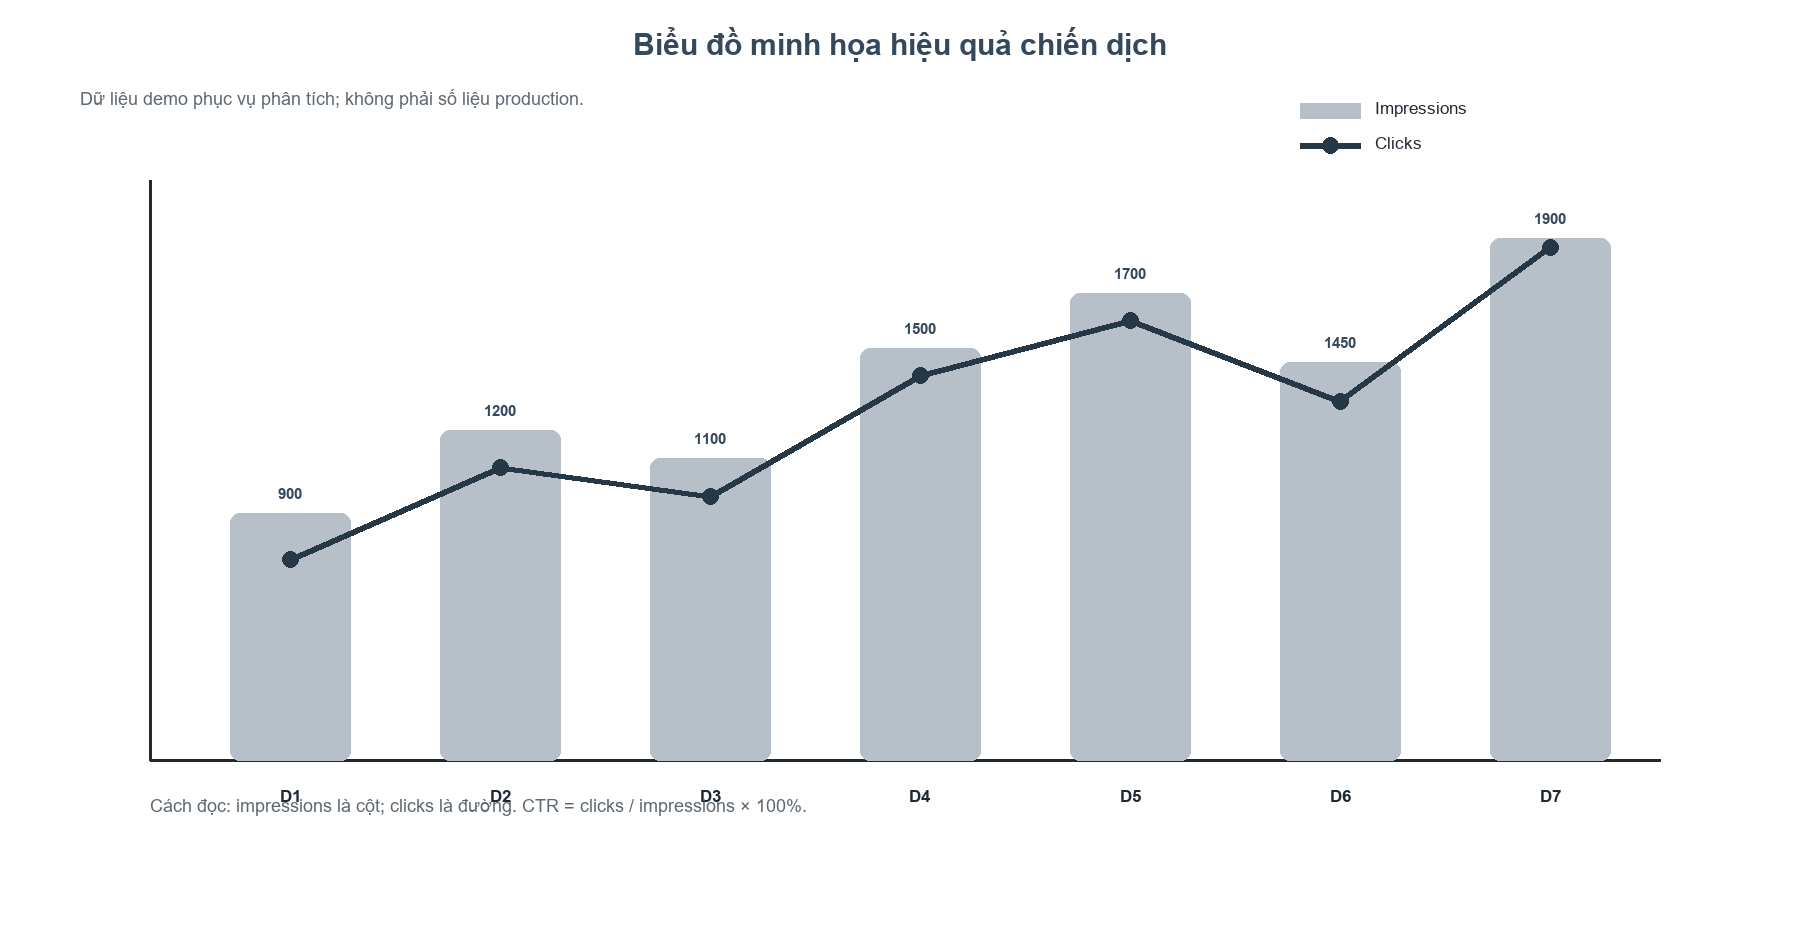
\includegraphics[width=0.88\linewidth]{metric-chart.png}
\caption{Biểu đồ minh họa impressions và clicks theo 7 ngày (dữ liệu demo)}
\end{figure}

% -------------------------------------------------------------------------
% NFR and use cases
% -------------------------------------------------------------------------
\section{Yêu cầu phi chức năng}
\begin{longtable}{@{}P{17mm}P{27mm}P{68mm}P{34mm}@{}}
\toprule
\tablehead{ID} & \tablehead{Nhóm} & \tablehead{Yêu cầu} & \tablehead{Cách xác minh}\\
\midrule
\endhead
NFR--001 & Security & authentication, authorization, CSRF, env secret, không commit API key & code review + test quyền\\
NFR--002 & AI safety & không bịa claim, không tự đăng, có warning & unit/integration test + review\\
NFR--003 & Data integrity & validation và unique constraint & model test/migration\\
NFR--004 & Availability & migrate/seed/run sạch; backup/restore có hướng dẫn & runbook + restore check\\
NFR--005 & Performance & CRUD p95 mục tiêu $<$2 giây/50 user; AI timeout 20 giây & target + timeout/fallback\\
NFR--006 & Authorization & Staff nhập; Manager duyệt/từ chối/đăng; route đều kiểm tra role & permission tests\\
NFR--007 & UX & status/filter/error/empty state rõ & manual/browser check\\
NFR--008 & Maintainability & module hóa app, prompt tách khỏi view & structure review\\
NFR--009 & Printability & A4; in trắng đen vẫn đọc được; màu không phải tín hiệu duy nhất & grayscale render check\\
\bottomrule
\end{longtable}

\subsection{Ma trận phân quyền}
\begin{tabularx}{\linewidth}{@{}Y P{35mm}P{35mm}@{}}
\toprule
\tablehead{Chức năng} & \tablehead{Marketing Staff} & \tablehead{Marketing Manager}\\
\midrule
Xem/tạo/sửa campaign & Có & Có\\
Quản lý channel & Có & Có\\
Tạo content và ghi metric & Có & Có\\
Duyệt/từ chối/đăng content & Không & Có\\
Xem thống kê và gọi AI & Có & Có\\
\bottomrule
\end{tabularx}

Backup SQLite, RPO/RTO và cách restore được ghi tại
\sourcefile{docs/12-operations-and-backup.md}.

\section{Use case}
\subsection{UC--01 -- Tạo chiến dịch}
\textbf{Actor:} Marketing Manager/Staff.\\
\textbf{Tiền điều kiện:} đã đăng nhập và có quyền.\\
\textbf{Luồng chính:} mở form -- nhập objective/audience/product/dates/budget --
hệ thống validate -- lưu campaign -- hiển thị chi tiết.\\
\textbf{Ngoại lệ:} ngày sai hoặc ngân sách âm -- báo lỗi, không lưu.\\
\textbf{Hậu điều kiện:} campaign có status và người tạo.

\subsection{UC--02 -- Sinh nội dung AI và duyệt}
\textbf{Actor:} Staff yêu cầu; Manager duyệt.\\
\textbf{Luồng chính:} chọn brief/kênh/giọng -- AI adapter tạo draft -- lưu/hiển
thị warning -- Manager kiểm tra -- approve hoặc reject -- chỉ approved mới
publish.\\
\textbf{Ngoại lệ:} provider lỗi/thiếu key -- fallback; thiếu dữ liệu -- warning.\\
\textbf{Hậu điều kiện:} content có source AI, prompt version và trạng thái duyệt.

\subsection{UC--03 -- Theo dõi hiệu quả}
\textbf{Actor:} Manager/Staff được cấp quyền.\\
\textbf{Luồng chính:} nhập metric theo ngày/kênh -- validate -- aggregate --
hiển thị views/clicks/conversions/cost/CTR/CPA.\\
\textbf{Ngoại lệ:} click vượt view hoặc conversion vượt click -- từ chối.

\begin{figure}[H]
\centering

\includegraphics[width=0.77\linewidth]{usecase.png}
\caption{Use Case của hệ thống}
\end{figure}

% -------------------------------------------------------------------------
% Data and architecture
% -------------------------------------------------------------------------
\section{Thiết kế dữ liệu}
\subsection{Bảng chính}
\begin{tabularx}{\linewidth}{@{}P{38mm}P{20mm}Y Y@{}}
\toprule
\tablehead{Bảng} & \tablehead{Khóa chính} & \tablehead{Khóa ngoại} & \tablehead{Ràng buộc}\\
\midrule
\sourcefile{campaigns_channel} & id & -- & name unique\\
\sourcefile{campaigns_campaign} & id & created\_by $\rightarrow$ User & budget $\geq$ 0, date range\\
\sourcefile{campaigns_content} & id & campaign, channel, approved\_by $\rightarrow$ User & status workflow\\
\sourcefile{campaigns_metric} & id & campaign, channel & unique campaign/channel/date; nonnegative\\
\bottomrule
\end{tabularx}

\subsection{Quan hệ}
\begin{itemize}
  \item Campaign 1--N Content.
  \item Campaign 1--N Metric.
  \item Channel 1--N Content.
  \item Channel 1--N Metric.
  \item User 1--N Campaign qua \code{created\_by} và 1--N Content qua \code{approved\_by}.
\end{itemize}

\begin{figure}[H]
\centering

\includegraphics[width=0.88\linewidth]{erd.png}
\caption{ERD -- có User, approved\_by và các quan hệ 1--N}
\end{figure}

\section{Kiến trúc hệ thống}
\begin{lstlisting}
Browser
  -> Django URLs/Views + auth/RBAC
  -> Forms/Services/validation
  -> Django ORM + SQLite
  -> Campaign/Channel/Content/Metric/User
  -> AI adapter (prompt version + provider/fallback + JSON validation)
  -> human approval gate
\end{lstlisting}

\begin{figure}[H]
\centering

\includegraphics[width=0.90\linewidth]{architecture.png}
\caption{Kiến trúc và luồng dữ liệu chính}
\end{figure}

\subsection{Mapping code}
\begin{tabularx}{\linewidth}{@{}P{18mm}P{43mm}Y P{31mm}@{}}
\toprule
\tablehead{Layer} & \tablehead{File} & \tablehead{Trách nhiệm} & \tablehead{Trạng thái}\\
\midrule
Config & \sourcefile{marketing_management/config/settings.py} & Django/SQLite/env & \baseline\\
Model & \sourcefile{campaigns/models.py} & entity, validation, aggregate, approval & \baseline\\
Form & \sourcefile{campaigns/forms.py} & input form & \baseline\\
Service & \sourcefile{campaigns/services.py} & create campaign transaction & \baseline\\
View & \sourcefile{campaigns/views.py} & \shortstack[l]{auth/list/create/detail/\\channel/metric/filter/\\dashboard/approval/AI} & \baseline\\
AI & \sourcefile{campaigns/ai_service.py} & prompt/provider/fallback/schema validation & \baseline\\
Test & \sourcefile{campaigns/tests.py} & 21 test model/permission/view/AI/CRUD/filter/dashboard/seed & \baseline\\
\bottomrule
\end{tabularx}

% -------------------------------------------------------------------------
% AI
% -------------------------------------------------------------------------
\section{Định vị AI}
\subsection{AI trong sản phẩm}
AI--001/002 hỗ trợ tạo draft; AI--003 có thể tóm tắt metric. AI không phải nguồn
sự thật của ngân sách/metric và không tự thay đổi dữ liệu.

\subsection{AI trong SDLC}
\begin{tabularx}{\linewidth}{@{}P{22mm}Y Y@{}}
\toprule
\tablehead{Giai đoạn} & \tablehead{Cách sử dụng} & \tablehead{Minh chứng}\\
\midrule
KT1 & phân tích actor, FR/NFR, ERD, vị trí AI & \sourcefile{docs/} + prompt review\\
KT2 & sinh model/CRUD/test/debug & 21 test + \code{manage.py check}\\
KT3 & thử prompt, kiểm tra schema/overclaim & \sourcefile{evidence/ai/AI-CAM-001-v1-review.md}\\
Cuối kỳ & tạo README/report/asset và review & PDF/LaTeX + checklist\\
\bottomrule
\end{tabularx}

\section{Prompt và AI contract}
\subsection{Prompt system}
\begin{quote}\small
\textbf{System:} Bạn là trợ lý marketing. Tạo nội dung nháp để con người duyệt; chỉ dùng
thông tin được cung cấp; không bịa cam kết, số liệu, giải thưởng hoặc chứng nhận;
không tự đăng. Nếu thiếu dữ liệu, nêu warning.
\end{quote}

\subsection{Prompt user}
\begin{quote}\small
Campaign brief: \texttt{\{\{campaign\_brief\}\}}\\
Objective: \texttt{\{\{objective\}\}}\\
Audience: \texttt{\{\{audience\}\}}\\
Product: \texttt{\{\{product\}\}}\\
Channel: \texttt{\{\{channel\}\}}\\
Tone: \texttt{\{\{tone\}\}}\\
Hãy đề xuất đúng 5 ý tưởng, mỗi ý tưởng gồm title, hook, draft và CTA.
\end{quote}

\subsection{Output contract}
\begin{lstlisting}
{
  "provider": "fallback|provider-name",
  "prompt_version": "AI-CAM-001-v1",
  "ideas": [{"title": "...", "channel": "...", "hook": "...",
             "draft": "...", "cta": "..."}],
  "requested_count": 5,
  "needs_human_approval": true,
  "warning": "..."
}
\end{lstlisting}
Backend chỉ nhận provider output khi có đúng 5 object đủ
\code{title/channel/hook/draft/cta}, đúng prompt version và approval flag; nếu
sai schema, timeout hoặc lỗi mạng thì dùng fallback.

% -------------------------------------------------------------------------
% Verification and Bài 2
% -------------------------------------------------------------------------
\section{Kiểm thử và minh chứng}
\subsection{Lệnh chạy local}
\begin{lstlisting}[language={bash}]
cd marketing_management
python -m venv .venv
.venv\Scripts\Activate.ps1
pip install -r requirements.txt
Copy-Item .env.example .env
python manage.py migrate
python manage.py seed_demo
python manage.py test campaigns -v 1
python manage.py runserver
\end{lstlisting}

Mở \code{http://127.0.0.1:8000/accounts/login/}. Tài khoản demo phải được tạo
bằng \code{createsuperuser} hoặc gán nhóm Marketing Manager/Marketing Staff
trong Django admin; repository không chứa mật khẩu mẫu.

\subsection{Kết quả kiểm chứng}
\begin{lstlisting}
python manage.py check                 -> no issues
python manage.py migrate --check       -> pass
python manage.py test campaigns -v 1   -> 21 tests, OK
python manage.py seed_demo              -> Demo marketing data is ready.
\end{lstlisting}

Các test bao phủ aggregate metric, approval gate, fallback AI, permission guard,
CRUD bốn nhóm dữ liệu, lọc keyword/channel/date/sort, filter sai không crash,
dashboard KPI, xử lý \code{ProtectedError}, staff bị chặn route manager-only và
\code{seed\_demo} idempotent/console-safe.

\subsection{Đối chiếu Bài kiểm tra thường xuyên 2}
Ma trận đầy đủ 10 tiêu chí nằm tại
\sourcefile{docs/13-bai-2-implementation.md}. Bảng sau tóm tắt bằng chứng trong
repository.

\begin{longtable}{@{}P{9mm}P{44mm}P{35mm}P{72mm}@{}}
\toprule
\tablehead{\#} & \tablehead{Tiêu chí} & \tablehead{Trạng thái} & \tablehead{Bằng chứng}\\
\midrule
\endhead
1 & Cấu trúc dự án hợp lý & \baseline & \sourcefile{config/}, \sourcefile{campaigns/}, templates, static, docs, requirements\\
2 & Đăng nhập và phân quyền & \baseline & auth URLs, \code{marketing\_access\_required}, \code{manager\_access\_required}, test staff bị chặn\\
3 & CRUD nghiệp vụ chính & \baseline & CRUD Campaign/Channel/Content/Metric; test update và POST delete\\
4 & Tìm kiếm, lọc, sắp xếp & \baseline & keyword, status, channel, date range, sort; ngày sai không crash\\
5 & Thống kê/báo cáo & \baseline & dashboard aggregate campaign/active/pending/clicks/cost\\
6 & Giao diện dễ dùng & \baseline & templates, CSS responsive, empty state, message, validation, confirm delete\\
7 & CSDL và dữ liệu mẫu & \baseline & SQLite, migration, seed demo, constraint; test seed idempotent\\
8 & Xử lý lỗi cơ bản & \baseline & validation, 400/405, protected delete và thông báo không crash\\
9 & Minh chứng AI lập trình & \baseline & \sourcefile{evidence/ai/B2-CODE-001-v1-review.md}\\
10 & Mã nguồn/tài liệu chạy thử & \baseline & README, \code{.env.example}, requirements, lệnh chạy/test; commit cuối cần chốt\\
\bottomrule
\end{longtable}

\subsection{Minh chứng sử dụng AI}
\sourcefile{evidence/ai/B2-CODE-001-v1-review.md} ghi input theo nguồn P0, phạm
vi hỗ trợ CRUD/filter/dashboard, file đã sửa, cách sinh viên kiểm chứng và giới
hạn. Phản hồi AI nghiệp vụ fallback được lưu riêng trong thư mục
\sourcefile{evidence/ai/} cùng JSON đã khử dữ liệu.

% -------------------------------------------------------------------------
% Risks and conclusion
% -------------------------------------------------------------------------
\section{Rủi ro và điểm mở}
\begin{tabularx}{\linewidth}{@{}P{19mm}Y P{20mm}Y@{}}
\toprule
\tablehead{ID} & \tablehead{Rủi ro/điểm mở} & \tablehead{Mức} & \tablehead{Cách xử lý}\\
\midrule
RISK--001 & Provider ngoài chưa test & Cao & fallback + mock/contract\\
RISK--002 & Overclaim/prompt injection & Cao & grounding + approval + redaction\\
RISK--003 & Ma trận quyền cần xác nhận & Trung bình & test quyền; chốt khi demo\\
RISK--004 & AI UI summary chưa có & Trung bình & giữ PROPOSED\\
RISK--005 & Tài liệu legacy & Cao & loại khỏi manifest\\
\bottomrule
\end{tabularx}

\section{Kế hoạch triển khai tiếp}
\begin{enumerate}
  \item Bổ sung audit log đầy đủ và các filter nghiệp vụ nâng cao.
  \item Thêm màn hình AI ideas và tạo Content từ draft với audit record.
  \item Thêm AI performance summary từ metric đã kiểm quyền.
  \item Thêm integration test provider mock, injection, PII, timeout và schema lỗi.
  \item Chốt commit cuối, chạy lại checklist và đóng gói PDF/LaTeX/ZIP.
\end{enumerate}

\section*{Kết luận}
\addcontentsline{toc}{section}{Kết luận}
Đề tài đúng của nhóm là \textbf{Hệ thống quản lý chiến dịch marketing có tích hợp
AI}, không phải hệ thống quản lý bán hàng. Hồ sơ đã xác định bối cảnh, actor,
FR/NFR, dữ liệu, kiến trúc, vị trí AI, prompt, approval gate, backup và minh
chứng phản hồi. Baseline code/test khớp với các trạng thái trong báo cáo;
provider thật và AI summary vẫn giữ nhãn PROPOSED/OPEN để bảo đảm trung thực học
thuật. Bài 2 được đối chiếu riêng theo 10 tiêu chí tại
\sourcefile{docs/13-bai-2-implementation.md}; điểm số cuối cùng vẫn do giảng viên
chấm.

\end{document}
